\documentclass[a4paper, 12pt]{article} % Статья формата A4, 12 шрифт
\usepackage{fontspec} % Для выбора шрифта
\usepackage[russian]{babel} % Поддержка русского языка
\setmainfont{Times New Roman}
\usepackage{graphicx} % Для вставки картинок
\usepackage{float} % Для точного расположения рисунков, таблиц
\usepackage{caption} % Для подписей к рисункам и таблицам
\usepackage{array} % Для улучшенной работы с таблицами
\usepackage{indentfirst} % Для красной строки в первом абзаце
\usepackage{geometry} % Пакет для настройки размера страницы и полей документа
\usepackage{wrapfig} % Для обтекания картинки текстом
\geometry{top=2cm, bottom=2cm, left=2cm, right=2cm}
\captionsetup{labelsep=period} % чтобы после "Рисунок 1" стояла точка

\begin{document}
	\noindent УДК 004.5
	
	\begin{flushright}
		А.А. Квашнин (1 курс), А.А. Земляк (1 курс),\\
		Г.А. Мирошник
	\end{flushright}
	
	\begin{center}
		\textbf{СМАРТ-УСТРОЙСТВА МОНИТОРИНГА СЕРДЕЧНО-СОСУДИСТОЙ СИСТЕМЫ (СУМССС)}
	\end{center}
	
	\textit{Введение.}
	В жизни человека одним из главных факторов является его
	здоровье, сохранность которого очень важна для любого из нас и всего общества в целом.
	Поэтому мы решили рассмотреть различные варианты по увеличению качества здравоохранения
	каждого человека на планете. Проведя исследования, мы поняли, что множество людей погибает
	или, остаются инвалидами из-за поздней индикации болезни. Главной причиной гибели
	являются сердечно-сосудистые заболевания (ССЗ). Поэтому, используя современные технологии
	программирования и автоматизации, мы решили разработать устройство, способное предупреждать
	человека об ухудшении в его здоровье, и по надобности привлекать постороннюю помощь.
	Мы рассмотрели основные актуальные области нашей работы:
	
	\textit{1.}
	Смертность - ССЗ являются основной причиной смерти во всем мире: ни по какой другой причине
	ежегодно не умирает столько людей, сколько от ССЗ. По оценкам, в 2012 году от ССЗ умерло 17,5
	миллиона человек, что составило 31\% всех случаев смерти в мире [1].
	
	\textit{2.}
	Доступность - Более 75\% случаев смерти от ССЗ происходят в странах с низким и средним уровнем доходах [1].
	
	\textit{3.}
	Своевременность: люди, страдающие ССЗ или подвергающиеся высокому риску таких заболеваний,
	нуждаются в раннем выявлении и оказании помощи путем консультирования и,
	при необходимости, приема лекарственных средств.
	
	\textit{4.}
	Реальность - на данный момент не существует компактного переносимого устройства,
	которое могло бы одновременно отслеживать параметры человека и предпринимать
	какие-то действия для улучшения его состояния.
	
	\textit{Цель работы.}
	Провести исследования по изучению причин и следствий изменения измеряемых параметров человеческого тела,
	влияния на них окружающей среды и внедрить полученные знания в программном обеспечении и прошивке устройства.
	Разработать дешёвое и удобное устройство с большим набором инструментов для отслеживания основных параметров человека
	и окружающей среды с низким энергопотреблением в компактном корпусе.
	
	Мы поставили перед собой ряд задач для достижения заданной цели:
	\begin{itemize}
		\item Изучить лидирующие причины смерти человека.
		\item Исследовать все возможные к получению физиологические данные человека и окружающей его среды.
		\item Выяснить причину изменения физиологических данных человека.
		\item Изучить влияние параметров окружающей среды на человека.
		\item Применить полученные знания на практике и реализовать программный софт.
		\item Изучить медицинские особенности этих болезней [1-3].
		\item Выполнить конечный этапный прототип устройства. Замерить энергопотребление.
		\item Протестировать устройство, снять показатели и провести их анализ.
	\end{itemize}
	
	\begin{center}
		\textbf{Режимы устройства}
	\end{center}
	
	\textit{Напоминания о принятии лекарств по расписанию}
	
	Режим помогает вовремя принимать необходимые лекарства и в случае, если человеку стало плохо,
	и часы могут установить причину, на экране крупным шрифтом написано название лекарства,
	которое необходимо принять человеку. Уведомление показано на рисунке 1.
	
	\begin{wrapfigure}{r}{0.42\textwidth}
		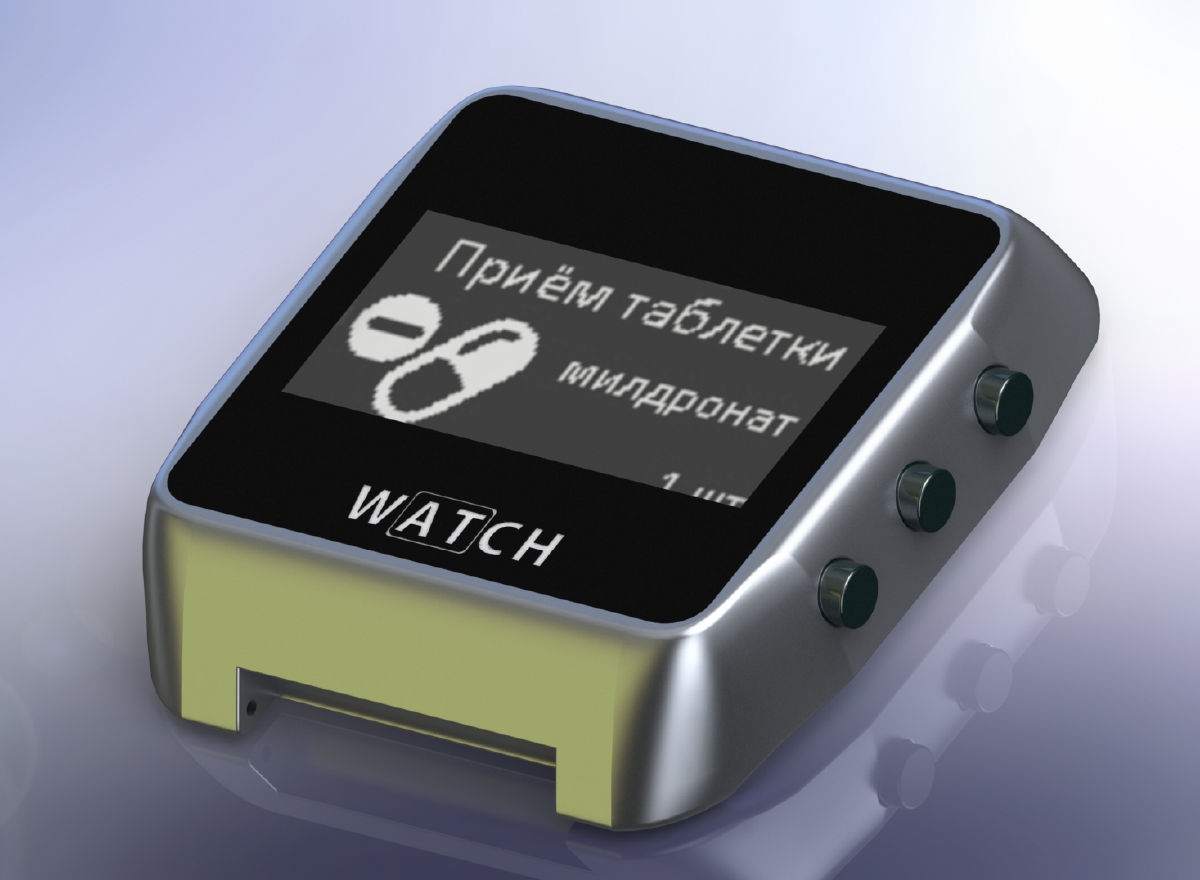
\includegraphics[width=0.42\textwidth]{image1.png}
		\caption{Уведомление о приеме лекарства}
	\end{wrapfigure}
	
	\textit{Срочная помощь}
	
	В случае если параметры человека вышли за пределы допустимых норм, то часы предпринимают
	меры по оповещению окружающих людей путём мигания экраном и звуковыми оповещениями.
	
	\textit{Активный режим}
	
	Режим, в ходе которого идёт повышенное наблюдение за всеми параметрами и их анализ в режиме реального времени.
	Повышенная скорость опроса всех датчиков в 4 раза. Специально для занятия спортом.
	
	\textit{Режим предупреждения}
	
	В случае если какой-либо из параметров человека стремится к критическому,
	часы уведомляют человека об этом и просят снизить нагрузку на организм.
	
	Помимо этих режимов есть главные циклы проверки, которые проверяют основные параметры человека.
	
	\begin{center}
		\textbf{Разработка}
	\end{center}
	
	\begin{wrapfigure}{r}{0.42\textwidth}
		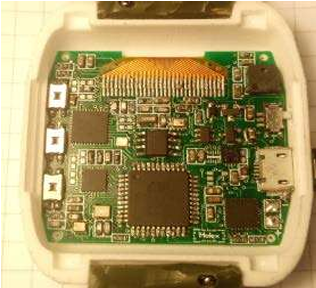
\includegraphics[width=0.42\textwidth]{image2.png}
		\caption{Печатная плата устройства}
	\end{wrapfigure}
	
	Печатная плата показана на рисунке 2, спроектирована в САПР Sprint Layout и содержит компоненты:
	ATMEGA1284p-au (Микроконтроллер с высоким функционалом и низким энергопотреблением),
	DS1337 (Часы реального времени),
	nrf24101 (Беспроводная передача данных),
	CP2102 (USB to UART преобразователь),
	мср73832 (Контроллер заряда аккумулятора),
	ХС6206Р252МR (Стабилизатор 2.8В с низким падением напряжения),
	ВМР280 (Барометр, гигрометр, термометр),
	MLT-5020 (пьезо-элемент),
	MAX30102 (Датчик сердцебиения и температуры кожи),
	LIS3DHTR (3х осевой акселерометр),
	UG-2864KSWLG01 (1.3in oled дисплей). Компоненты, расположенные на одной стороне печатной платы с целью уменьшения габаритов устройства [4-5].
	
	Прошивка состоит из Arduino совместимого bootloader и основной программы.
	Прошивка занимает 31 Кбайт постоянной памяти, оставшееся место выделено под хранение данных суточного мониторинга,
	которые можно считать на компьютере по средствам USB [6].
	
	Полученные данные можно открыть в специальной программе, написанной на языке C++ в среде Visual Studio.
	
	\begin{table}[H]
		\centering
		\caption{Анализ существующих решений}
		\begin{tabular}{|m{4.4cm}|m{2.8cm}|m{3cm}|m{2.2cm}|m{2cm}|}
			\hline
			\textbf{Параметры сравнения} & \textbf{Холтер} & \textbf{Имплант} & \textbf{Смарт устройства} & \textbf{СУМССС} \\
			\hline
			Точность выявления болезней & Высокая & Очень высокая & Низкая & Высокая \\
			\hline
			Диапазон выявляемых болезней & Очень высокая & Низкая & Очень низкая & Высокая \\
			\hline
			Максимальное время автономного мониторинга & 7 дней & Больше года & 2 дня & 24 дня \\
			\hline
			Удобство использования & Низкая & Высокая & Высокая & Высокая \\
			\hline
			Цена & 20000-400000 рублей & От 500000 рублей & От 1000 рублей & 2000 рублей \\
			\hline
		\end{tabular}
	\end{table}
	
	\textit{Результаты.}
	В заключение нам удалось создать рабочий прототип устройства,
	которое позволяет отслеживать основные показатели человека и вовремя предупреждать его в случае опасности.
	Постобработка полученных данных поможет в выявлении проблем со здоровьем человека.
	Устройство заряжается по USB, что показано на рисунке 3.
	
	\begin{wrapfigure}{r}{0.42\textwidth}
		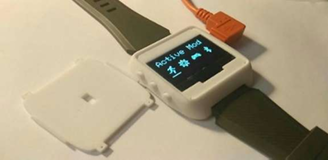
\includegraphics[width=0.42\textwidth]{image3.png}
		\caption{Зарядка устройства по USB}
	\end{wrapfigure}
	
	\textit{Вывод.}
	На данный момент устройство способно выявлять аритмию, фибрилляцию желудочков,
	коронарную недостаточность, гипертрофию миокарда, стенокардию, инфаркт миокарда.
	
	Благодаря низкому энергопотреблению устройством можно пользоваться на протяжении длительного времени без дополнительной подзарядки.
	
	Маленькие размеры и форма часов удобны в повседневном использовании.
	
	Данные часы помогут уменьшить смертность людей, а также сформировать базу данных проблем со здоровьем и условий, при которых они возникают.
	
	\begin{thebibliography}{6}
		\bibitem{1}
		Макаров Л.М. Национальные российские рекомендации по применению методики холтеровского мониторирования
		в клинической практике // Российский кардиологический журнал. – 2014. - №2 (106). – С. 6-61.
		\bibitem{2}
		Франклин Циммерман. Клиническая электрокардиография. - 2017 г. – 423 с.
		\bibitem{3}
		Ю.В. Щукин. Электрокардиография. – Изд-во: Феникс, 2014 г. – 223 с.
		\bibitem{4}
		Майер Р.В. Основы электроники. Курс лекций: Учебно-методическое пособие. - Глазов: ГГПИ, 2011. - 80 с.
		\bibitem{5}
		Никулин С.А., Повный А.В. Энциклопедия начинающего радиолюбителя. -
		Изд-во: Наука и техника, 2011 г. - 384 с.
		\bibitem{6}
		В.Н. Баранов. Применение микроконтроллеров AVR: схемы, алгоритмы, программы
		/ 2-е изд., [испр.]. – М. Изд-во: Додэка-XXI, 2006 (М. : Типография "Новости"). - 287 с
	\end{thebibliography}
\end{document}